\newcommand\tab[1][1cm]{\hspace*{#1}}s
\begin{answer}
\\ \\
a) It takes 211  Failures before it converges. \\ \\
b) \begin{center}
  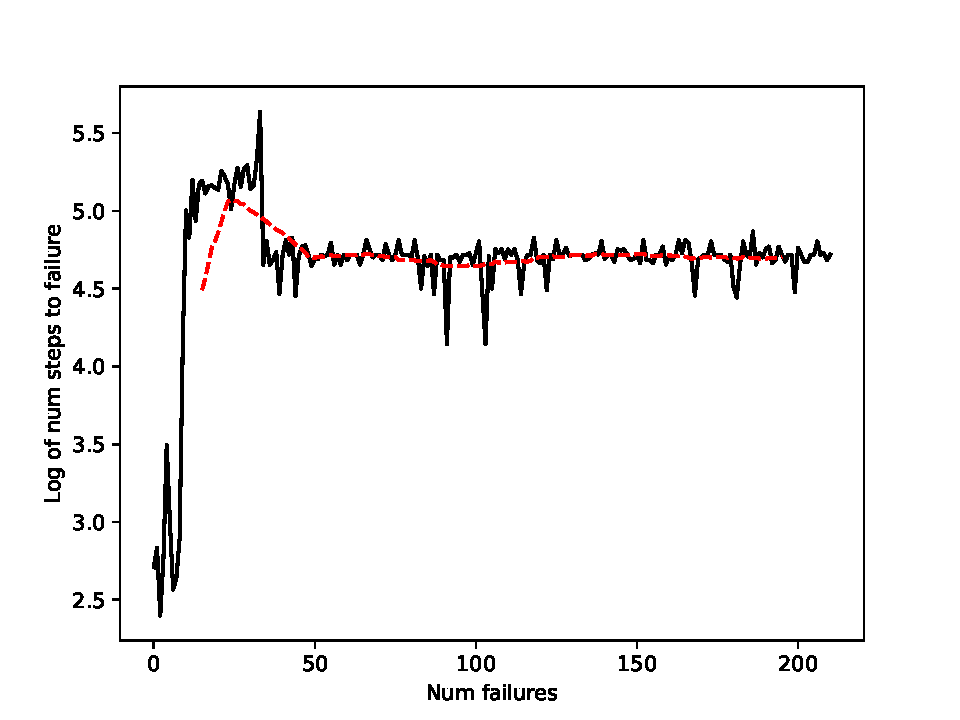
\includegraphics[width=6cm]{cartpole/control.pdf}
\end{center}

c) Seeds:
\tab 1 = 499 Failures \\ 
\tab 2 = 355 Failures \\ 
\tab 3 = 247 Failures \\ 
By looking at this very number of Failures and more, we can see that np and used in code generates random 1 and 0 which is set by this so this is will give different Faliures if seed is not set. \\ \\
\\ \\
\end{answer}